\section{Weltenmodell/Perception}
\subsection{Einleitung}
\frame
{\frametitle{Einleitung}
\begin{itemize}
    \item Warum brauchen wir denn so ein Modell?
    \item Was muss modelliert werden?
\end{itemize}
}

\subsection{Datenstrukturen}
\subsubsection{Die verschiedenen Entitäten}

\frame
{\frametitle{Feste Objekte}
\begin{center}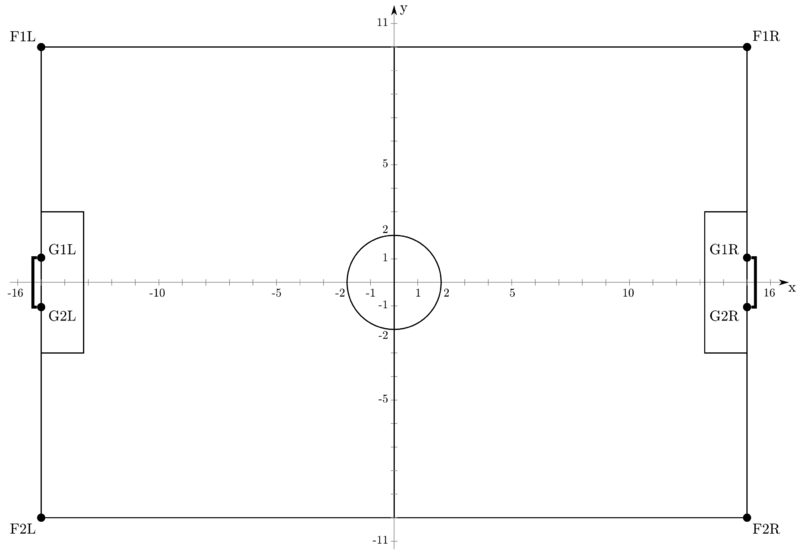
\includegraphics[height=6.3cm, center]{800px-SoccerSimulation_FieldPlan.png}\end{center}
\url{http://simspark.sourceforge.net/wiki/index.php/File:SoccerSimulation_FieldPlan.png}
}
%verschiedenste Linien, Pfosten, Eckfahnen, wobei die letzteren beiden eindeutig erkannt werden.

\frame
{\frametitle{Mobile Objekte}
\begin{center}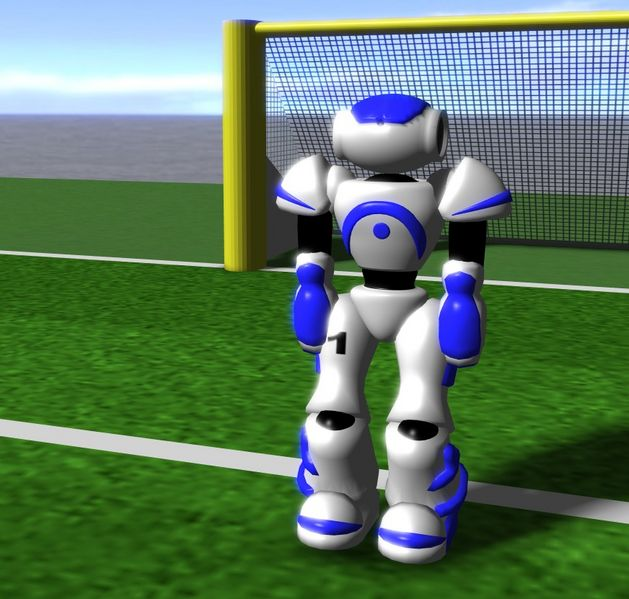
\includegraphics[height=6.3cm, center]{629px-Models-nao.jpg}\end{center}
\url{http://simspark.sourceforge.net/wiki/index.php/File:Models-nao.jpg}		%mal sebst noch nen cooleren Snapshoot machen ...
}
%Spieler, Ball
\subsubsection{Modellierung}
\frame
{\frametitle{Klassenmodell des Gegenstandbereiches}
\begin{center}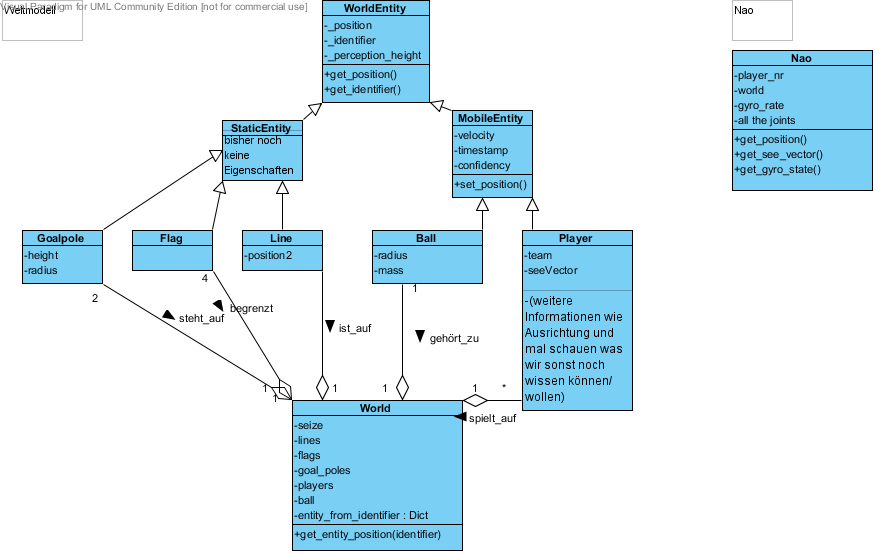
\includegraphics[height=6.3cm, center]{Weltenmodell.png}\end{center}
}

\subsection{Lokalisierung}

\subsubsection{Selbstlokalisierung}
\frame
{\frametitle{Probleme bei der Berechnung}
%\begin{gather*}
(See ($<$name$>$ (pol $<$distance$>$ $<$angle1$>$ $<$angle2$>$))\\
\hspace*{8mm}(P (team $<$teamname$>$) (id $<$playerID$>$)\\
\hspace*{13mm}($<$bodypart$>$ (pol $<$distance$>$ $<$angle1$>$ $<$angle2$>$)))\\
\hspace*{8mm}(L (pol $<$distance$>$ $<$angle1$>$ $<$angle2$>$) \\
\hspace*{13mm}(pol $<$distance$>$ $<$angle1$>$ $<$angle2$>$)))
%\end{gather*}
\begin{center}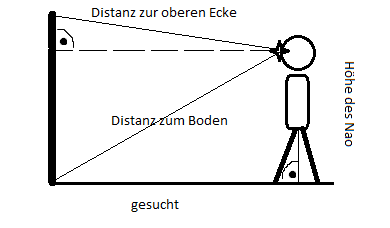
\includegraphics[height=3.5cm, center]{Distanz_3D_Kugelkoordinaten_zu_2D_kartesisch.png}\end{center}
$gesucht = \sqrt{\textbf{Distanz}^2 - (\textbf{Objekthöhe} - \textbf{Augenhöhe des Naos})^2}$
}
%3d polar zu 2D kartesisch
%verschied

\frame
{\frametitle{Positionsbestimmung}
\begin{center}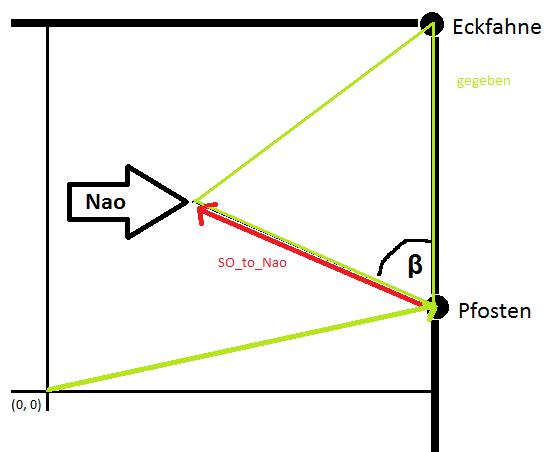
\includegraphics[height=4.5cm, center]{Positionsbestimmung.png}\end{center}%hübscheres Bild ...
Kosinussatz für beliebige Dreiecke: $b^2 = a^2 + c^2 - 2ac \cos (\beta)$
}
%Wir brauchen immer 2 Objekte!

\subsubsection{Blickrichtung}
\frame
{\frametitle{Blickrichtung (See-Vektor)}
\begin{itemize}
    \item für jede wahrgenommene statische Entität:
	\begin{itemize}
	    \item Vektor Kamera $\rightarrow$ Entität konstruieren
	    \item ins Sichtzentrum des NAOs rotieren
	\end{itemize}
    \item arithmetisch mitteln und fertig
\end{itemize}
}

\subsubsection{Lokalisation mobiler Entitäten}
\frame
{\frametitle{Lokalisation mobiler Entitäten}
\begin{itemize}
    \item sozusagen die Rückrichtung
    \item für jede wahrgenommene mobile Entität:
	\begin{itemize}
	    \item den See-Vektor nehmen
        \item auf die Distanz zur Entität skalieren
        \item in die wahrgenommene Richtung der Entität rotieren
        \item NAO-Position + Vektor = Entität-Position
	\end{itemize}
\end{itemize}
}

\frame
{\frametitle{Rauschen und Abschätzung der Genauigkeit}
Echte Wahrscheinlichkeitsverteilung:
\begin{center}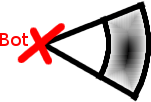
\includegraphics[height=2.1cm, center]{MPGI3-RC-13S_Wahrscheinlichkeit1.png}\end{center}
Damit lässt es sich aber nicht angenehm rechnen... \\
Also 
\begin{center}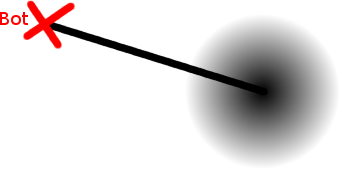
\includegraphics[height=2.1cm, center]{MPGI3-RC-13S_Wahrscheinlichkeit2.png}\end{center}
}